\begin{frame}
\frametitle{Vertex Buffer: Demo}
\begin{figure}[ht]
    \centering
    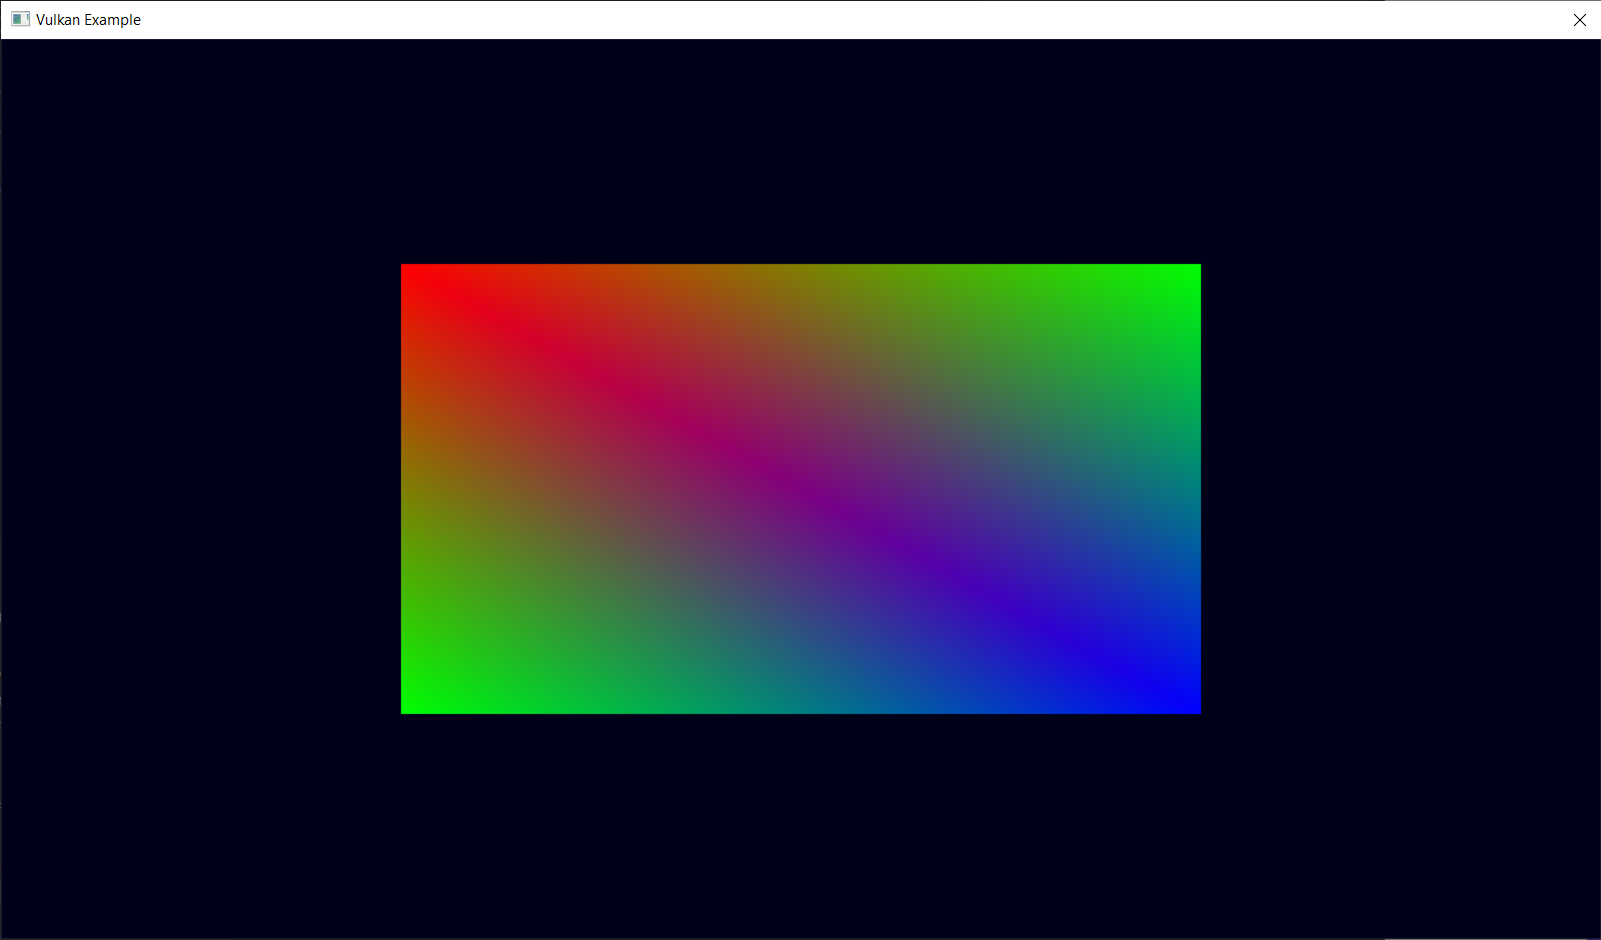
\includegraphics[scale=0.25]{images/SlidesVertices/RenderQuad.png}
\end{figure}
\end{frame}

\begin{frame}
\frametitle{Vertex Buffer}
\begin{itemize}
\item I nostri vertici sono in RAM e noi dobbiamo caricarli nella memoria della GPU
\item I vertici non cambiano durante l'esecuzione dell'applicazione
\item Vogliamo rendere la lettura dei nostri vertici, da parte della GPU, il più veloce possibile
\item Usiamo due buffer
\item Uno staging buffer, allocato su memoria della GPU host visible (lenta)
\item Scriviamo i dati dei nostri vertici su questo buffer
\item Un vertex buffer, allocato su memoria della GPU device local (veloce)
\item Inviamo un comando alla GPU per trasferire il contenuto dello staging buffer nel vertex buffer
\end{itemize}
\end{frame}
